\section{Artificial neural networks}

An \gls{ann} is a computational model used in computer science, machine learning, and other research areas. \glspl{ann} are loosely modeled after the human brain. The human brain contains vast amounts of nerve cells (neurons), which are highly interconnected, creating a huge network of signal transmission. Each neuron receives an electric signal from all the cells it is connected to (its neighbours). If the signal reaches a certain threshold, the neuron sends a signal on to all its neighbours. The procedure repeats itself, propagating electric signals throughout the brain.

Similarly to the human brain, \glspl{ann} are built up by connecting a set of simple units called \textit{perceptrons}. \footnote{Perceptrons are often referred to as neurons or nodes. In the context of \glspl{ann}, the three are interchangeable.} A perceptron takes in up to several weighted input values. The input values are summarized, usually together with a weighted constant, called the \textit{bias}. The summed inputs are fed into a function, called the \textit{activation function}. The result of the activation function is called the perceptron \textit{output}. The equation for a perceptron can be written as
\begin{equation*}
    y = K \left(\sum_{i = 1}^{n} w_{i}x_{i} + w_{0}b \right),
\end{equation*}
where $y$ is the perceptron output, $K$ the activation function, $n$ the number of incoming connections, $x_{i}$ and $w_{i}$ the value and weight of the $i^{\text{th}}$ incoming connection, and $b$ and $w_{0}$ the perceptron's bias and bias weight. The value of $b$ is usually $-1$ or $1$.

Perceptrons are usually connected in several \textit{layers} with various topologies (see \cref{subsec:network-types}). In \glspl{ann}, the electric signals are replaced with sets of real valued numbers, called the network \textit{input}. The input travel from the first (input) layer, possibly via intermediate (hidden) layers to the last (output) layer. An example of a simple two-layer \gls{ann} is shown in \cref{fig:network-layers-example}.

\begin{figure}
    \centering
    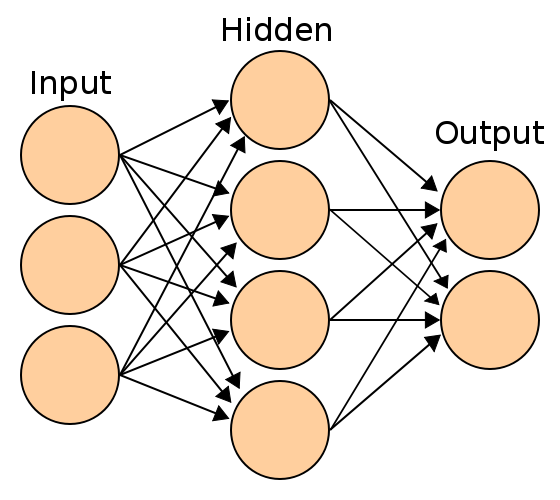
\includegraphics[width=0.5\textwidth]{artificial-neural-networks/network-layers-example.png}
    \caption{Example of a simple two-layer feedforward artificial neural network. By Colin M. L. Burnett, distributed under a CC BY-SA 3.0 license.}
    \label{fig:network-layers-example}
\end{figure}

Changing the number of layers, number of perceptrons in each layer, or the layer topologies can have huge impacts on how well the network perform, and what it can learn. Another important parameter of an \gls{ann} is the perceptrons' activation functions. The activation function determines what signal the perceptron outputs. There are countless available functions to use. The \gls{tanh} function, sigmoid function, softplus function \citep{bib:glorot2011deep}, and the \gls{relu} \citep{bib:nair2010rectified} are popular choices.

\subsection{Network structures}
\label{subsec:network-types}

There are several ways to organize the layers of an \gls{ann}, depending on what the network is trying to learn. Below is a description of two commonly used network structures that are used later in this report.

\subsubsection{\glspl{fnn}}

An \gls{fnn} is the simplest type of \gls{ann}. In an \gls{fnn}, the signals move forwards from the input through the output. Each perceptron in one layer is fully connected to all perceptrons in the subsequent layer. An example of an \gls{fnn} is shown in \cref{fig:network-layers-example}.

\subsubsection{\glspl{rnn}}

Unlike the connections in an \gls{fnn}, the connections in an \gls{rnn} can form cyclic graphs. An \gls{rnn} contains at least one feed-back connection, i.e. a connection that forms a loop. This creates an internal state of the network, allowing the network to incorporate a form of memory.

The internal memory of \glspl{rnn} make them extra useful in processing sequences of inputs, such as speech recognition.


\subsection{The training procedure}

There are several ways of training an \gls{ann}. One of the most popular training methods is called back-propagation. The method consists of two main phases: forward-propagation of input signals, and backward-propagation of error gradients.

In the forward-propagation phase, input values are fed through the input nodes and propagated through the network, generating an output. The generated output is then compared to the target output, using the \textit{loss function}. A loss function calculates the difference between the generated output and the desired output in some way. The \gls{mse} and \gls{mae} are examples of such functions.

In the backward-propagation phase, the output errors propagate backwards through the network, calculating an error gradient value for each neuron in the hidden layers. The neuron gradients are fed into the \textit{optimization function}. An optimization function adjusts the neuron weights in order to minimize the loss function. A common way of minimizing the cost function is through methods using \textit{gradient descent}. \cref{fig:gradient-descent-example} shows an example of the progression of the gradient descent method applied to a 2D function. Methods using gradient descent adjust the weights in order to "descend" the loss function towards a minimum. Popular methods utilizing gradient decent include \textit{stochastic gradient descent} \citep{bib:bottou2010large}, \textit{RMSProp} \citep{bib:hinton2012neural}, and \textit{Adam} \citep{bib:kingma2014adam}.

\begin{figure}
    \centering
    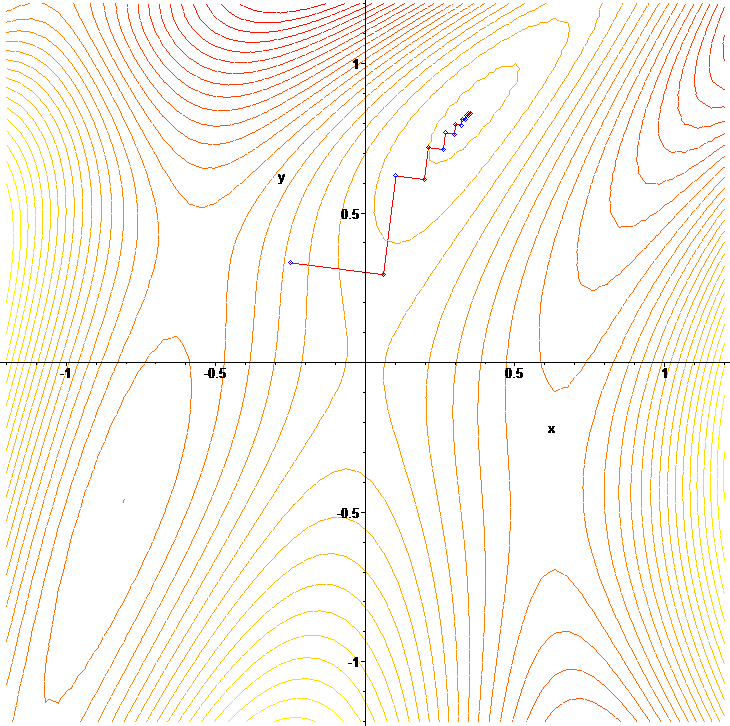
\includegraphics[width=0.7\textwidth]{artificial-neural-networks/gradient-descent-example.png}
    \caption{Example of the gradient descent method applied to a 2D function. By Joris Gillis.}
    \label{fig:gradient-descent-example}
\end{figure}

By iterating the back-propagation cycle, the weights eventually converge towards the target function. That is, if the input values are sufficient in order to describe the target function. The neurons in the hidden layers organize themselves so that they learn to recognize the patterns of the input space. Then, if a noisy, unknown observation appears, the network can respond properly if the observation contains the same underlying patterns as a training example.


\subsubsection{Dropout}

\glspl{ann} are, as other classification methods, prone to overfitting. Dropout is a widely used method for avoiding overfitting \citep{bib:srivastava2014dropout}. Using dropout, for each node, there is a probability $p$ that the node will be "deactivated", set to zero and not evaluated during training. \cref{fig:network-dropout} shows an \gls{ann} where dropout is applied.

The back-propagation method builds up co-adaptations for the training data. These adaptations do not generalize to unobserved data. Dropout breaks up these adaptations by making the presence of a specific hidden unit unreliable \citep{bib:srivastava2014dropout}.

\begin{figure}
    \centering
    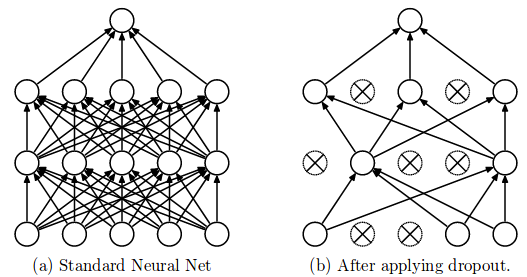
\includegraphics[width=0.7\textwidth]{artificial-neural-networks/dropout.png}
    \caption{Graphical illustration of the effects of dropout. Taken from \citet{bib:srivastava2014dropout}.}
    \label{fig:network-dropout}
\end{figure}